\documentclass[twocolumn,10pt,a4paper]{article}
\usepackage[margin=0.75in]{geometry}
\usepackage[utf8]{inputenc}
\usepackage[T1]{fontenc}
\usepackage{lmodern}
\usepackage{microtype}
\usepackage{cite}
\usepackage{url}
\usepackage{hyperref}
\usepackage{xcolor}
\usepackage{enumitem}
\usepackage{tabularx}
\usepackage{booktabs}
\usepackage{tikz}
\usetikzlibrary{positioning,arrows.meta,fit,calc}
\hypersetup{colorlinks=true,citecolor=blue,linkcolor=blue,urlcolor=blue}

\title{Paper 3: Fixture-Driven Research Harness for Falsifiable O-RAN Remediation Claims}

\author{David Kypuros \\
\small Red Hat \\
\small \texttt{dkypuros@redhat.com}}

\date{31 May 2026}

\begin{document}
\maketitle

\begin{abstract}
Paper 3 in this five-paper series describes the fixture-driven research harness that makes covered v0 claims falsifiable. Agentic-AI-for-networks papers frequently make architectural claims that are difficult to falsify because the implementation is proprietary, partially specified, or not runnable independently. We describe the research engineering methodology behind a closed-loop Day-2 remediation harness for O-RAN Cloud RAN that takes the opposite posture: every covered v0 implementation claim anchors to a file or fixture, every authored harness or scenario YAML/JSON file carries citation metadata, and a verify gate produces a binary pass/fail result a reviewer can reproduce against a cited repository state. The methodology has four anchoring layers (citation headers, JSON Schema contracts, a bidirectional standards-lineage index, and end-to-end fixture replay) and an explicit stub-boundary discipline that names which components carry the paper's claims and which exist only to isolate the real components from external dependencies. Full ten-check reproduction requires jsonschema; without it, schema validation is reported as skipped. The LLM-neutral design is enforced structurally rather than by convention, which preserves determinism in the verify gate. We argue this style of research substrate produces bounded, falsifiable outputs independent of LLM provider, API availability, or model-version drift.
\end{abstract}

\section{Introduction}

For a software harness to serve as a research substrate (as opposed to a product prototype), it should produce bounded claims that a reviewer can falsify mechanically. Three properties matter: covered v0 implementation claims are anchored to specific files, the substrate runs reproducibly without external dependencies, and stub boundaries are declared rather than hidden. The dominant pattern in agentic-AI-for-networks publications fails one or more of these properties. Implementations are described in prose without file-level anchors; the runtime depends on a live cloud, a live cluster, or a particular API key; and the stub boundary (the line between code under test and the systems being mocked) is implicit.

A prior multivendor diagnostic publication \cite{multivendor_blog_2026} established a fault-localization substrate for Cloud RAN troubleshooting. The closed-loop extension we describe in companion papers takes the same posture: the research artifact is the runnable open-source repository, the architectural narrative is anchored at file plus line, and the verify gate is the falsification mechanism. This paper documents the methodology by which the three substrate properties are achieved. The repository under discussion is open-source under Apache-2.0 at \url{https://github.com/dkypuros/oran-agent-harness}.

The remainder of the paper is organized as follows. Section \ref{sec:anchoring} documents the four-layer claim anchoring system. Section \ref{sec:gate} describes the verify gate's ten possible checks and the failure mode each one guards. Section \ref{sec:stub} describes the stub-boundary discipline. Section \ref{sec:llm} describes the LLM-neutral design as a research methodology requirement, not only a production concern. Section \ref{sec:compare} compares the approach to adjacent research engineering practices. Section \ref{sec:repro} states the reproducibility entry point. Section \ref{sec:conclude} concludes.

\section{The Claim Anchoring System}
\label{sec:anchoring}

\begin{figure}[t]
\centering
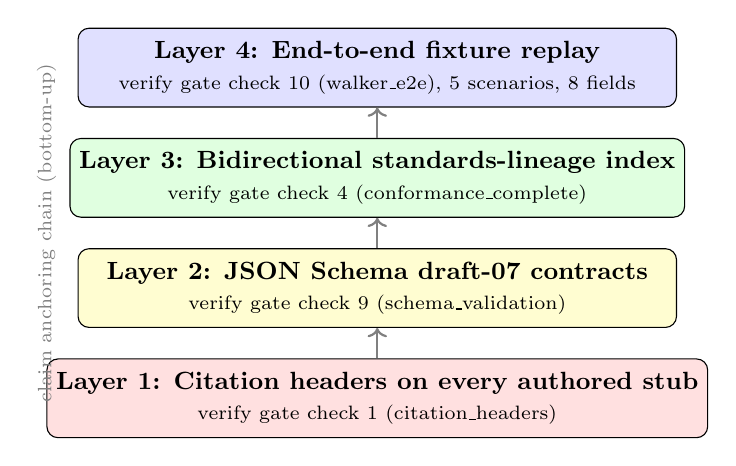
\begin{tikzpicture}[
  layer/.style={draw, rounded corners, minimum width=7.6cm, minimum height=1.0cm, font=\small, align=center},
  l1/.style={layer, fill=red!12},
  l2/.style={layer, fill=yellow!18},
  l3/.style={layer, fill=green!12},
  l4/.style={layer, fill=blue!12},
  arr/.style={->, thick, gray}
]
\node[l4] (l4) at (0, 3.6) {\textbf{Layer 4: End-to-end fixture replay}\\ \scriptsize verify gate check 10 (walker\_e2e), 5 scenarios, 8 fields};
\node[l3] (l3) at (0, 2.2) {\textbf{Layer 3: Bidirectional standards-lineage index}\\ \scriptsize verify gate check 4 (conformance\_complete)};
\node[l2] (l2) at (0, 0.8) {\textbf{Layer 2: JSON Schema draft-07 contracts}\\ \scriptsize verify gate check 9 (schema\_validation)};
\node[l1] (l1) at (0, -0.6) {\textbf{Layer 1: Citation headers on every authored stub}\\ \scriptsize verify gate check 1 (citation\_headers)};

\draw[arr] (l1.north) -- (l2.south);
\draw[arr] (l2.north) -- (l3.south);
\draw[arr] (l3.north) -- (l4.south);

\node[font=\scriptsize, rotate=90, gray] at (-4.2, 1.5) {claim anchoring chain (bottom-up)};
\end{tikzpicture}
\caption{Four-layer claim anchoring system (read bottom-up). Each layer is mechanically enforced by a specific check of the verify gate when optional dependencies are installed. Layer 1 turns documentation into a repository contract; Layer 4 turns covered v0 routing, action, and reversibility claims into mechanically falsifiable assertions against committed expected outputs.}
\label{fig:fourlayer}
\end{figure}

Four layers of anchoring carry the load. Figure~\ref{fig:fourlayer} shows the layered hierarchy.

\subsection{Layer 1: Citation headers on every stub}

Every YAML and JSON file authored under \texttt{harness/} and \texttt{scenarios/} opens with a \texttt{\_conforms\_to} or equivalent block naming the spec lineage, the spec section, the spec version, and the bibliography reference numbers. The verify gate's first check enforces this: any new file added without a citation header fails the gate. The mechanism turns documentation into a repository contract. Adding a routing rule, a schema, a guardrail, or a scenario fixture without naming its lineage is a build failure, not a documentation oversight.

\subsection{Layer 2: JSON Schema draft-07 contracts}

Five harness-authored schemas define the shapes the pipeline produces and consumes: \texttt{FaultPayload.json}, \texttt{RCA.json}, \texttt{RemediationProposal.json}, \texttt{AuditEvent.json}, and \texttt{ReversibilityProfile.json}. With jsonschema installed, each scenario's \texttt{fault\_payload.json} validates against \texttt{FaultPayload.json}; each scenario's embedded remediation object validates against \texttt{RemediationProposal.json}; and each embedded reversibility profile validates against \texttt{ReversibilityProfile.json}. The gate's ninth check runs those validations. A claim like "the audit event always carries a populated reversibility profile" stops being a prose assertion and becomes a schema-shape validation outcome. The full TMF688 audit envelope remains a harness-authored shape claim, not a standards-body certification.

\subsection{Layer 3: Bidirectional standards-lineage index}

A single file \texttt{harness/conformance.md} is a two-column table mapping every authored artifact in the harness tree to its spec lineage and bibliography references. The gate's fourth check confirms both directions: every file under \texttt{harness/} or \texttt{scenarios/} appears in the table, and every row in the table points at a file that exists. The mechanism prevents the index from rotting silently as the codebase changes. A new file without an entry fails the gate; an entry pointing at a deleted file fails the gate. This is traceability of standards-lineage metadata, not formal conformance certification.

\subsection{Layer 4: End-to-end fixture replay}

The gate's tenth check runs the deterministic walker as a subprocess against all five committed scenario fault payloads. For each scenario, the actual audit event output is compared against the committed expected audit event on eight material comparisons: seven named fields (\texttt{targetLayer}, \texttt{taxonomyMatch}, \texttt{actionType}, \texttt{ocloudInternalPath}, \texttt{actionPayloadRef}, \texttt{dryRun}, \texttt{requiresHumanApproval}) plus the \texttt{reversibility\_profile.confidence\_in\_reversibility} sub-field comparison. Any divergence on any comparison fails the gate. The mechanism turns selected v0 claims about routing decisions, action types, and the seven-field reversibility contract into mechanically falsifiable assertions.

\section{The Verify Gate}
\label{sec:gate}

\begin{figure*}[t]
\centering
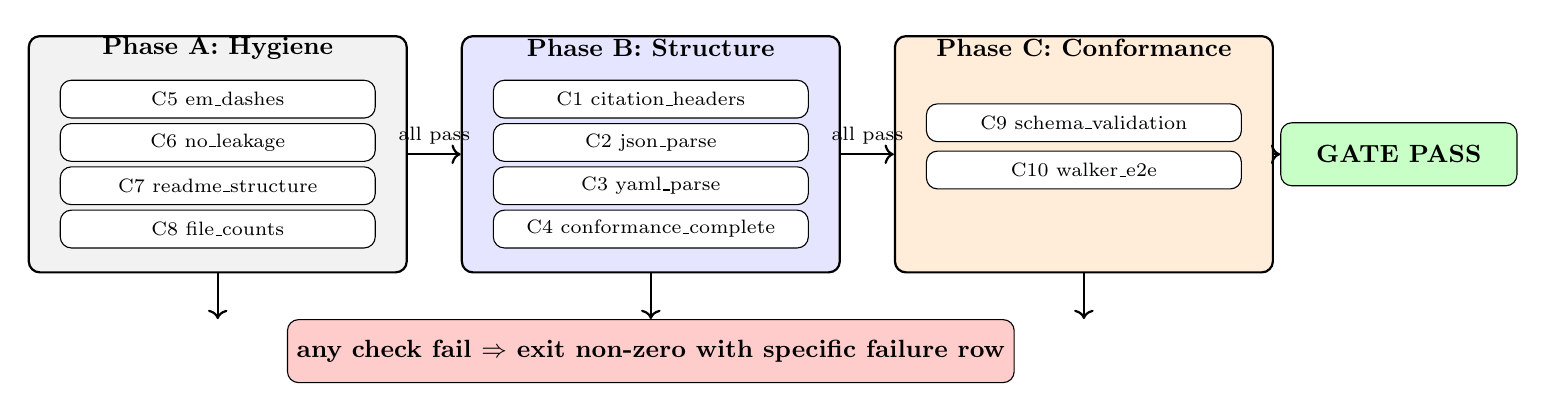
\begin{tikzpicture}[
  phase/.style={draw, rounded corners, thick, minimum width=4.8cm, minimum height=3.0cm, align=center},
  check/.style={draw, rounded corners, fill=white, minimum width=4.0cm, minimum height=0.48cm, font=\scriptsize, align=center},
  pass/.style={draw, rounded corners, fill=green!22, minimum width=3.0cm, minimum height=0.8cm, font=\small\bfseries, align=center},
  block/.style={draw, rounded corners, fill=red!20, minimum width=8.0cm, minimum height=0.8cm, font=\small\bfseries, align=center},
  arr/.style={->, thick}
]
\node[phase, fill=gray!10]   (pa) at (0, 0)   {};
\node[phase, fill=blue!10]   (pb) at (5.5, 0) {};
\node[phase, fill=orange!15] (pc) at (11, 0)  {};

\node[font=\small\bfseries] at (0, 1.35)   {Phase A: Hygiene};
\node[font=\small\bfseries] at (5.5, 1.35) {Phase B: Structure};
\node[font=\small\bfseries] at (11, 1.35)  {Phase C: Conformance};

\node[check] at (0, 0.7)  {C5 em\_dashes};
\node[check] at (0, 0.15) {C6 no\_leakage};
\node[check] at (0, -0.4) {C7 readme\_structure};
\node[check] at (0, -0.95){C8 file\_counts};

\node[check] at (5.5, 0.7)  {C1 citation\_headers};
\node[check] at (5.5, 0.15) {C2 json\_parse};
\node[check] at (5.5, -0.4) {C3 yaml\_parse};
\node[check] at (5.5, -0.95){C4 conformance\_complete};

\node[check] at (11, 0.4)  {C9 schema\_validation};
\node[check] at (11, -0.2) {C10 walker\_e2e};

\draw[arr] (pa.east) -- node[above, font=\scriptsize] {all pass} (pb.west);
\draw[arr] (pb.east) -- node[above, font=\scriptsize] {all pass} (pc.west);

\node[pass] (gp) at (15, 0) {GATE PASS};
\draw[arr] (pc.east) -- (gp.west);

\node[block] (bk) at (5.5, -2.5) {any check fail $\Rightarrow$ exit non-zero with specific failure row};
\draw[arr] (pa.south) -- (bk.north -| pa.south);
\draw[arr] (pb.south) -- (bk.north);
\draw[arr] (pc.south) -- (bk.north -| pc.south);

\end{tikzpicture}
\caption{Ten-check verify gate as a three-phase pipeline when optional schema validation is available. Phase A enforces hygiene (em-dash audit, leakage guard, README structure, file counts). Phase B enforces structural integrity (citation headers, JSON and YAML parse, standards-lineage index). Phase C enforces schema-shape and fixture-replay integrity (JSON Schema validation, end-to-end walker replay). Any executed check failure exits the gate non-zero with a specific failure row.}
\label{fig:verifygate}
\end{figure*}

The gate is a single Python script at \texttt{scripts/verify.py}. With PyYAML and jsonschema installed, it runs ten checks in sequence and exits 0 on 10 of 10 pass, non-zero with specific failure rows otherwise. Without jsonschema, check 9 is reported as skipped and the reduced gate reports the executed checks. Figure~\ref{fig:verifygate} shows the three-phase pipeline. Table~\ref{tab:verify-claims} maps each check to the bounded claim it supports, the evidence inspected, and the limit that remains outside the v0 claim. Each check guards a specific failure mode.

\begin{table*}[t]
\centering
\small
\begin{tabularx}{\textwidth}{p{1.2cm}X X X}
\toprule
Check & Claim bounded by the gate & Evidence inspected & Limit \\
\midrule
C1 & Authored harness and scenario YAML/JSON files carry standards-lineage metadata & \texttt{\_conforms\_to} keys or citation headers under \texttt{harness/} and \texttt{scenarios/} & Metadata presence, not standards-body certification \\
C2 & Public JSON files are syntactically parseable & JSON parser over the public tree & Syntax only, not semantic correctness \\
C3 & Public YAML files are syntactically parseable & PyYAML parser over the public tree & Syntax only, not policy correctness \\
C4 & The standards-lineage index is bidirectionally complete & \texttt{harness/conformance.md} rows compared against files under \texttt{harness/} and \texttt{scenarios/} & Only indexed repository artifacts are covered \\
C5 & The public tree satisfies the manuscript's em-dash hygiene rule & Unicode scan for U+2014 & Style hygiene only \\
C6 & Tracked files do not include the configured leakage patterns & \texttt{git ls-files} checked for forbidden paths and PDFs outside allowed paper outputs & Not a general secret scanner \\
C7 & The README keeps the expected public entry structure & Line-count bounds and three required lede strings & Structure check, not full documentation audit \\
C8 & The public harness surface has not silently expanded or shrunk & Fixed counts for \texttt{harness/} and skill markdown files & Intentional scope growth requires updating the gate \\
C9 & Scenario payloads and embedded remediation objects match harness-authored schemas & \texttt{jsonschema} validation of fault payloads, remediation objects, and reversibility profiles & Optional dependency; schemas are harness-authored research contracts \\
C10 & The deterministic walker reproduces covered v0 routing, action, and reversibility outcomes & Subprocess replay of five committed scenarios against expected audit fixtures on eight material comparisons & Partial scenario coverage over stubbed partner-system inputs \\
\bottomrule
\end{tabularx}
\caption{Claims proven by the verify gate. Each row states the bounded claim, the evidence the script inspects, and the limit that should remain visible in the manuscript. The table prevents the phrase "verify gate pass" from being read as live O-RAN, TM Forum, Kubernetes, Redfish, or LLM interop.}
\label{tab:verify-claims}
\end{table*}

\textbf{Check 1, citation\_headers.} Guards against undocumented stubs. A new YAML or JSON file added without a \texttt{\_conforms\_to} block fails the check.

\textbf{Check 2, json\_parse.} Guards against syntax rot in any JSON file across the public tree.

\textbf{Check 3, yaml\_parse.} Same for YAML files.

\textbf{Check 4, conformance\_complete.} Bidirectional standards-lineage index integrity (Layer 3 above).

\textbf{Check 5, em\_dashes.} Guards against a specific authorship tell that the author has committed to eliminating from published copy. The check reports zero permitted occurrences of the em dash codepoint (U+2014) in the public tree.

\textbf{Check 6, no\_leakage.} Guards against accidentally committing \texttt{.env} files, \texttt{.local/} content, credentials, or large local demo artifacts. Runs against \texttt{git ls-files} so it catches anything the working tree might hide.

\textbf{Check 7, readme\_structure.} Guards against the README drifting from the three stated repository goals. Enforces line-count bounds and the presence of the three-goal lede.

\textbf{Check 8, file\_counts.} Guards against silent file additions or deletions that change the harness surface without updating the index. The count is asserted at known totals.

\textbf{Check 9, schema\_validation.} Scenario fault payloads and embedded remediation plus reversibility subobjects validate against the harness-authored JSON Schemas (Layer 2 above). The check is required for a full ten-check reproduction and auto-skips if the \texttt{jsonschema} package is not installed, with a warning.

\textbf{Check 10, walker\_e2e.} The falsifiability check (Layer 4 above). Spawns the walker as a subprocess, captures the audit event, compares to the committed expected output on material fields.

Run-time of the entire gate against the reference repository state is approximately five seconds on a developer-grade workstation. The dependency surface is Python 3.8 or later, PyYAML, and (optionally) jsonschema. No cloud account, no live cluster, no LLM API key is required for the deterministic gate.

\section{Stub Boundary Discipline}
\label{sec:stub}

The harness is explicit about what is real and what is stubbed. The methodology argument is that the components carrying the paper's claims must be real; the components that exist only to isolate them from external dependencies should be stubbed cleanly.

\textbf{Real components.} The \texttt{harness/runtime/router.py} module performs the deterministic taxonomy lookup against the authored \texttt{harness/taxonomy.yaml}. It is exercised end-to-end in check 10 of the verify gate. The \texttt{harness/runtime/guardrail.py} module evaluates the five-subcheck policy guardrail against the authored \texttt{harness/guardrails.yaml}. Both modules' deterministic behavior is the source of the paper's claims about routing and gating. They are real Python code executing real YAML inputs.

The repository also ships a real Python function call that exercises an O2-IMS-shaped adapter boundary from the architecture diagram: \texttt{5G\_O-RAN\_SIM/oam/o2ims\_stub.py}'s \texttt{deploy\_request} function is invoked by the router on every infrastructure-layer route, and the response envelope is attached to the audit. The stub is shape-only (no network call, no real reconcile loop), but the function call is real, and the test \texttt{test\_o2ims\_dispatch\_attached\_on\_down\_route} asserts that the response shape is contract-correct.

\textbf{Stubbed components.} The Agentic Gateway, the four MCP servers (\texttt{mcp-platform}, \texttt{mcp-ran}, \texttt{mcp-hardware}, \texttt{mcp-ocloud}), the three domain agents (Platform, RAN, Hardware), and the Digital Twin substrate are stubbed. The walker's module docstring names them directly. The stub boundary is declared, not hidden. Each scenario's canned values (RCA timestamp, contributing signals, action target, blast radius, sandbox verdict, SMO dispatch outcome, O2 IMS dispatch outcome) live in a single file at \texttt{harness/runtime/scenario\_stubs.json}, which serves as the explicit single source of truth for stubbed data.

This design decision matters for the research substrate property. The real components (router, guardrail, o2ims function call) are the ones that carry the paper's architectural claims, and they are exercised against authored YAML and JSON inputs the verify gate validates. The stub components are wrappers that isolate the real components from external dependencies (a live MCP server, a live LLM endpoint, a live Twin cluster) so the gate can run without network access, credentials, or vendor-specific tooling. A reviewer can change the stubbed inputs and observe the real components' deterministic response.

\section{The LLM-Neutral Substrate as a Research Property}
\label{sec:llm}

The harness's third declared contribution is an LLM-neutral substrate. The motivation is partly production-pragmatic (avoid lock-in to a specific provider) but the research methodology value is stronger.

If the runtime embedded a specific LLM provider's SDK or a specific model identifier, the verify gate's tenth check (walker end-to-end) would have nondeterministic output. Different reviewers running the gate against the same repository state at the same git SHA would see different outcomes depending on provider availability, model version, or even response-time jitter. The research substrate property would collapse.

The harness enforces LLM neutrality structurally rather than by convention. The routing rule's ambiguous path raises \texttt{NotImplementedError} in the default code path, preserving determinism in the verify gate. The live LLM path is gated behind an environment variable (\texttt{ORAN\_LLM\_MODE=live}) and a separate test (\texttt{test\_route\_ambiguous\_with\_llm\_mode\_live}) that skips by default to keep the gate result independent. Provider reachability for Anthropic, the OpenAI API, or an OpenAI-compatible on-premises vLLM endpoint is tested separately by \texttt{scripts/test\_llm\_live\_path.py}; it is not part of the committed scenario replay. The structural enforcement means a reviewer cannot accidentally make the gate provider-dependent.

The LLM is therefore not load-bearing on the routing decision the verify gate proves. This is the right division of labor for a research substrate: the deterministic claims are reproducible at compile time, the LLM-assisted claims are gated behind a separate execution mode that does not interfere with the deterministic gate. A v1 deployment that wants real LLM behavior on the ambiguous path can light up the env-gated seam without touching the deterministic core.

\section{Comparison to Adjacent Research Practices}
\label{sec:compare}

Three adjacent research engineering practices illustrate the niche the harness occupies.

\textbf{Unit tests without spec-anchored fixtures.} Most research code ships with tests that confirm internal consistency (a function returns what its signature promises) but not external spec lineage or shape compatibility. The harness's check 10 binds the test output to committed expected audit fixtures, and those fixtures themselves validate against harness-authored, spec-cited JSON Schemas when jsonschema is installed. A change that breaks a covered v0 routing, action, or reversibility claim breaks the gate.

\textbf{Integration tests against live services.} Some research projects integration-test against a live cluster or API. This is honest about end-to-end behavior but defeats reproducibility: a reviewer without the live service cannot rerun the test. The harness preserves end-to-end coverage through fixture replay against committed canned inputs, which a reviewer can re-execute on a clean clone.

\textbf{Pure simulation.} Some research uses simulators that never touch real code paths through standardized interfaces. The harness occupies a middle position: the deterministic routing and guardrail logic are real Python executing real YAML; the simulated component is the partner system (the O-Cloud Manager, the partner SMO, the BMC) which is stubbed at the shape-correct envelope boundary. A v1 deployment can swap the stubs for live targets behind the same envelope.

\section{Reproducibility Entry Point}
\label{sec:repro}

A reader who wants to reproduce the full harness verify gate runs four commands.

\begin{verbatim}
git clone \
  https://github.com/dkypuros/oran-agent-harness
cd oran-agent-harness
pip install pyyaml jsonschema
python3 scripts/verify.py
\end{verbatim}

That is the complete reproducibility claim for the deterministic gate. No cloud account, no live cluster, and no LLM API key are required. The reference manuscript state is repository commit \texttt{a2686f42755ac9a0be27f3f97c5d142d6315047a}, dated 2026-05-31. At that referenced state, a clean clone with PyYAML and jsonschema installed is the state intended by the paper's \texttt{SUMMARY: 10/10 checks passed} and \texttt{OVERALL: PASS} claim. In reduced environments, \texttt{scripts/verify.py} reports check 9 as skipped and prints the executed-check denominator; dirty local working trees can fail hygiene checks independently of the referenced manuscript state.

Beyond the gate, the repository ships two lab postures. The macOS posture at \texttt{macbook\_lab/} uses Docker Desktop and a multi-container compose file to stand up a fuller stack with HTTP wrappers around the platform stubs. The Linux posture at \texttt{linux\_lab/} uses podman 5.4.1 on Fedora 42 with the same compose file. A verified run document at \texttt{linux\_lab/verified\_runs/2026-05-31\_fedora42\_podman.md} captures the live cross-runtime verification.

These lab postures are reviewer aids, not replacements for the deterministic proof. They expose the same fixtures through browser and chat surfaces, while the publication-grade falsification claim remains the clone, install, and \texttt{scripts/verify.py} path above.

\section{Reviewer-Operability Instrumentation}
\label{sec:discover}

The deterministic verify gate is the publication-grade falsification mechanism. The repository also ships a separate operator-facing inspection surface at \texttt{omc-skills/oran-discover/}. This surface is methodological instrumentation: it helps a reviewer or operator inspect the same state the papers discuss, but it is not the mechanism that proves the covered v0 claims.

The bundle consists of six read-only probes plus one orchestrator: \texttt{/oran-discover:ptp} for PTP and Cloud Notification state, \texttt{/oran-discover:metal3} for BMO and HostFirmwareComponents state, \texttt{/oran-discover:redfish} for BMC task state, \texttt{/oran-discover:smo} for TMF921 companion-intent state, \texttt{/oran-discover:taxonomy} for the 20-entry routing taxonomy, \texttt{/oran-discover:guardrail} for policy and crisis-mode state, and \texttt{/oran-discover:plan} as the pre-flight walk over the other six. The conformance index at \texttt{omc-skills/oran-discover/conformance.md} maps each skill to its live wrapper, static fallback file, and reference lineage.

The MacBook dashboard adds a reviewer-operable front door around that bundle. A reviewer can open the simple two-loop demo, request \texttt{/commands} to list the scoped slash-command surface, run \texttt{/oran-discover:plan} as a pre-flight survey, switch among \texttt{D\_phc\_drift\_hw\_only}, \texttt{E\_nic\_firmware\_update}, and \texttt{E\_with\_smo\_reject}, and attach a \texttt{harness-walker} sidecar via \texttt{/run/\{scenario\}} to display the live \texttt{AuditEvent}. With an assistant key configured, the chat harness can then summarize what the event proves and what remains blocked behind the operator. That explanation is convenience instrumentation; it may depend on the local lab and model configuration, whereas the deterministic verify gate does not.

A separate check at \texttt{scripts/test\_oran\_discover\_skills.py} verifies that the seven skill markdown files have the required structure, that their static source files exist, and, when the MacBook lab wrappers are running, that the live endpoints return the expected JSON keys. This complements \texttt{scripts/verify.py}. The verify gate proves bounded implementation claims through schemas and fixture replay; the discovery-skill check proves that the human-facing read-before-write surface is wired and documented.

\section{Honest Scope}

The methodology produces falsifiable claims for the bounded set of behaviors the verify gate covers. Several explicit limits.

\textbf{Fixtures are canned.} Scenario inputs and the partner-system stubbed responses do not come from a running O-Cloud or a real linuxptp daemon. A real cluster could produce inputs that fail validation against the JSON Schemas; that would be informative but is out of scope for the gate.

\textbf{Schemas are harness-authored.} The JSON Schema draft-07 contracts at \texttt{harness/schemas/} are the harness's own approximations of the spec envelopes. The schemas are not published by O-RAN, TM Forum, or any other standards body. A real spec-conformance test would use the standards bodies' own test suites (for example the O-RAN SC compliance test suite \cite{oran_sc_it_test}); that is a v1 work item.

\textbf{Scenario coverage is partial.} The five committed scenarios cover the primary delivery path branches (MCO, KMM, Metal3, dual-route accepted, dual-route SMO-rejected) but 15 of the 20 taxonomy entries have no walkthrough fixture. A future research artifact could claim broader coverage once those fixtures exist.

\textbf{Some signals are stubbed values.} EvalOps confidence telemetry, Agentic Recoverability validation history, the full Digital Twin convergence envelope, and partner-system responses are described in the architectural narrative and the schemas but populated as stubbed values in \texttt{scenario\_stubs.json} for v0. Live LLM provider reachability is a separate optional test, not a committed scenario fixture. Their real-time operation is a v1 deliverable.

\section{Conclusion}
\label{sec:conclude}

This paper has described the research engineering methodology behind a closed-loop Day-2 remediation harness for O-RAN Cloud RAN. Four anchoring layers (citation headers, JSON Schema contracts, a bidirectional standards-lineage index, fixture replay) and a verify gate make covered v0 implementation claims mechanically falsifiable. The stub boundary is declared, not hidden, and the components carrying the paper's claims are real code exercised against authored inputs. LLM neutrality is enforced structurally, which preserves verify-gate determinism. The combination produces a research substrate that any reviewer can reproduce on a clean clone in under five seconds when dependencies are installed. We argued this is a meaningful improvement over agentic-AI publications that ship prose architectural claims without spec-anchored falsification mechanisms. v0 limits are declared; the v1 path is named.

\section*{Acknowledgements}

The methodology builds on a prior multivendor diagnostic substrate co-authored with S. Kiani Mehr, N. Korati Prasanna, M. Vazquez Cebrian, S. Srikanthan, and P. Venkatesh \cite{multivendor_blog_2026}. Source code is Apache-2.0 licensed at \url{https://github.com/dkypuros/oran-agent-harness}.

\bibliographystyle{plain}
\bibliography{refs}

\end{document}
